%-----------------------------------------------------------------------------
%
%               Template for sigplanconf LaTeX Class
%
% Name:         sigplanconf-template.tex
%
% Purpose:      A template for sigplanconf.cls, which is a LaTeX 2e class
%               file for SIGPLAN conference proceedings.
%
% Guide:        Refer to "Author's Guide to the ACM SIGPLAN Class,"
%               sigplanconf-guide.pdf
%
% Author:       Paul C. Anagnostopoulos
%               Windfall Software
%               978 371-2316
%               paul@windfall.com
%
% Created:      15 February 2005
%
%-----------------------------------------------------------------------------


\documentclass[preprint]{sigplanconf}

% The following \documentclass options may be useful:

% preprint      Remove this option only once the paper is in final form.
% 10pt          To set in 10-point type instead of 9-point.
% authoryear    To obtain author/year citation style instead of numeric.

% !TEX root =  RefactorToCloud.tex

\usepackage{xspace}
\usepackage{graphicx}
\usepackage{amsmath}
\usepackage{color}
\usepackage[hidelinks]{hyperref}


%\usepackage[english]{babel}
%\usepackage{threeparttable}
%\usepackage{amssymb}
%\setcounter{tocdepth}{3}
%
%\usepackage{multirow}
%\usepackage{url}
%\usepackage{array}
%
%\usepackage{moreverb}
%\usepackage{listings}

%%\usepackage{cite}
%\usepackage{relsize}
%\usepackage{wasysym}
%\usepackage{fancybox}
%\usepackage{balance}
%\usepackage{enumitem}
%\usepackage{lmodern}
%\usepackage{caption}
%\usepackage{epstopdf}
%
%\usepackage[font={bf}, labelfont=bf]{caption}
%\usepackage[font={bf,small},labelfont=bf]{caption}
%\usepackage{datetime}

%\captionsetup[table]{skip=5pt}
%
%\newcommand{\version}[1]{\normalsize{Version #1 - \mydate\today\xspace,\xspace\currenttime}}
%
%\newdateformat{mydate}{\monthname[\THEMONTH]\xspace\THEDAY}
%
%\newcommand{\fixme}[1]{}
\newcommand{\TODO}[1]{\textcolor{magenta}{\textbf{TODO: }#1}}

%\newcommand{\FB}[1]{\textcolor{blue}{\textbf{FEEDBACK: }#1}}
\newcommand{\FB}[1]{{#1}}
%
%\newcommand{\ADD}[1]{\textbf{\textcolor{blue}{#1}}}
%\newcommand{\REMOVE}[1]{\textbf{\textcolor{red}{#1}}}
%
%\newcommand{\mybox}[1]{
%\begin{center}
%\setlength{\fboxsep}{5pt}%
%\Ovalbox{%
%\begin{minipage}{.45\textwidth}
%\begin{center}
%{\it #1} 
%\end{center}
%\end{minipage}}
%\end{center}
%}
%
%
%\lstdefinelanguage{TouchDevelop}
%{
%sensitive=true,
%morekeywords=[1]{
%var, add, if, private, action, returns, for, each, do, where},
%morecomment=[l]{//},
%morecomment=[s]{/*}{*/},
%morecomment=[l][keywordstyle4]{\#},
%morestring=[b]",
%morestring=[b]',
%}
%%
%%\DeclareCaptionFormat{listing}{\rule{\dimexpr\textwidth+17pt\relax}{0.4pt}\par\vskip1pt#1#2#3}
%%\captionsetup[lstlisting]{singlelinecheck=false, margin=0pt, font={sf},labelsep=space,labelfont=bf}
%%\renewcommand\lstlistingname{Code}
%%
%\definecolor{mygreen}{rgb}{0,0.6,0}
%\definecolor{mygray}{rgb}{0.5,0.5,0.5}
%\definecolor{mymauve}{rgb}{0.58,0,0.82}
%%
%\lstset{ %
%%frame=bottom,
%  language=TouchDevelop,                % the language of the code
%  basicstyle=\ttfamily\scriptsize,           % the size of the fonts that are used for the code
%  keywordstyle=\color{blue},
%  commentstyle=\color{mygreen},
%  numberstyle=\tiny\color{mygray}
%  stringstyle=\color{mymauve},
%  rulecolor=\color{black}, 
%  stepnumber=1,                   % the step between two line-numbers. If it's 1, each line 
%  %numbers=left,                   % where to put the line-numbers
%  numberstyle=\scriptsize,  
%  numbersep=5pt,  
%  showspaces=false,               % show spaces adding particular underscores
%  showstringspaces=false,         % underline spaces within strings
%  showtabs=false,                 % show tabs within strings adding particular underscores
%  tabsize=2,                      % sets default tabsize to 2 spaces
%  breaklines=false,                % sets automatic line breaking
%  breakatwhitespace=false,        % sets if automatic breaks should only happen at whitespace
%  belowskip=1pt,
%  aboveskip=2pt
%}
%
%
\newcommand{\codesnippet}[1]{
\begin{lstlisting}#1\end{lstlisting}}
%
%\newcommand{\readme}[1]{\texbf{ReadMe: }#1}
%
%\newcommand{\etal}{\emph{et~al}.~}
%\newcommand{\Comment}[1]{}%\textbf{\textsl{$\langle\!\langle$#1$\rangle\!\rangle$}}}
%\newcommand{\spacedinlineheader}[1]{\vspace{1.5 mm} \noindent \textbf{#1}}
%\newcommand{\Space}[1]{}


\newcommand{\numScripts}{116\xspace}
\newcommand{\numManual}{20\xspace}
\newcommand{\numFormative}{four\xspace}
\newcommand{\MT}{\begin{small}\textsc{Mileage Tracker}\end{small}\xspace}
\newcommand{\numTransformations}{2722\xspace}
\newcommand{\percentRefactored}{94\%\xspace}
%\newcommand{\TD}{TouchDevelop\xspace}
\newcommand{\TD}{\textsf{touch\textbf{develop}}\xspace}
\newcommand{\NC}{\code{Number Collection}\xspace}
\newcommand{\CDT}{\code{Cloud Data Table}\xspace}

\newcommand{\POne}{\textbf{(P1)}\xspace}
\newcommand{\PTwo}{\textbf{(P2)}\xspace}

\newcommand{\code}[1]{\begin{small}\texttt{#1}\end{small}}
%\newcommand{\URL}[1]{\begin{footnotesize}\url{#1}\end{footnotesize}}


\newcommand{\tool}{\begin{small}\textsc{Cloudifyer}\end{small}\xspace}



%\newcommand{\RQOne}{\textbf{RQ1:} How do developers use asynchronous programming?\xspace}
%
%\newcommand{\MisuseOne}{\subParagraph{(1) Fire \& Forget methods:}\xspace}








%Are they \textbf{safer} than manual approach?\xspace}
%Do they improve \textbf{code quality}?\xspace}

%\newcommand{\subParagraph}[1]{\textbf{\emph{#1}}}
\newcommand{\myParagraph}[1]{\noindent \textbf{#1}}








\usepackage{listings}
\usepackage{color}
\usepackage{xspace}
\usepackage{alltt}

 \usepackage{multirow} 
 \usepackage{rotating}
%%%%%%%%%%%%%%%%%%%%%%%%%%%%%%%%%%%%%%%%%%%%%%%%%%%%%%%%%%%%%%%%
%%%% THIS BELOW COPIED FROM vkuncak/doc/vmcai09/defs.tex
\definecolor{gray}{RGB}{211,211,211}
\newcommand{\jbasicstyle}{\scriptsize\sffamily}%\footnotesize}
\newcommand{\textcode}[1]{{#1}} % with current font \sf and \tt look ugly
\newcommand{\jnumberstyle}{\tiny}
\newcommand{\Hilight}{\makebox[0pt][l]{\color{gray}\rule[-3pt]{0.80\linewidth}{9pt}}}
\newcommand{\CodeIn}[1]{{\small\texttt{#1}}}

\newcommand{\codex}[1]{{\smaller\texttt{#1}}\xspace}

\newcommand{\tilted}[1]{\begin{turn}{75}#1\end{turn}}

\lstdefinelanguage{pseudo}
 {
%alsoletter={<>:=},
  morekeywords={int,boolean,new,continue,enum,
                void,if,else,while,return,for,foreach,in,assert,assume,false,true,class,static,import,
                ignoreIf,getInt,getAny,getNew,getExisting,getBoolean,force,concrete,Susp,
                getInt,getAny,getNew,getBoolean,force,concrete,Susp,max,min,ObjectPool,
                implements,interface,public,double,synchronized,final,
                proc,@Event,@Schedule,extends,case,sleep,waitForTick,assertTick,instanceof},
  keywordstyle=\bfseries,
  lineskip=-0.1em,
%  numbers=left,
  numbers=none,
  numberstyle=\jnumberstyle,
  numbersep=4pt,
%  basicstyle=\scriptsize,
  basicstyle=\jbasicstyle,
  breaklines=true,
  breakautoindent=true,
  tabsize=2,
%  columns=fixed,
%  columns=flexible,
  columns=fullflexible,
%  morecomment=*[s][\textsl]{/*:}{*/},
  morecomment=*[l][\textsl]{//},
%  morecomment=*[s][\jahobform]{"}{"},
  mathescape=true,
%  escapeinside=<>,
%  escapebegin={\begin{isakeyword}},
%  escapeend={\end{isakeyword}}
%  caption={},
%  label={},
}
\newcommand{\MyParagraph}[1]{\noindent \textbf{#1}}
\newenvironment{CodeOut}{\begin{scriptsize}}{\end{scriptsize}}



\newcommand{\vertbar}{vertBar\xspace}




\newcommand{\NumProjects}{9\xspace}
\newcommand{\NumSLOCReduced}{2213\xspace}
\newcommand{\NumOperationsInferred}{2681\xspace}
\newcommand{\NumChainsInferred}{1709\xspace}
\newcommand{\NumSLOCChangedAnon}{3707\xspace}
\newcommand{\NumSLOCChangedFor}{12313\xspace}
\newcommand{\NumSLOCChanged}{16020\xspace}


\usepackage{subfigure}
\usepackage{graphicx}
\usepackage{algorithm}
\usepackage{algpseudocode}
\usepackage{url}
\usepackage{footnote}
%\usepackage{biblatex}
%\usepackage{natbib}
\usepackage{balance}

\usepackage{float}
\restylefloat{table}





%\usepackage{hyperref}
%\pagenumbering{arabic}

\begin{document}

\thispagestyle{empty}
\pagenumbering{arabic}


\special{papersize=8.5in,11in}
\setlength{\pdfpageheight}{\paperheight}
\setlength{\pdfpagewidth}{\paperwidth}

\conferenceinfo{CONF 'yy}{Month d--d, 20yy, City, ST, Country} 
\copyrightyear{20yy} 
\copyrightdata{978-1-nnnn-nnnn-n/yy/mm} 
\doi{nnnnnnn.nnnnnnn}

% Uncomment one of the following two, if you are not going for the 
% traditional copyright transfer agreement.

%\exclusivelicense                % ACM gets exclusive license to publish, 
                                  % you retain copyright

%\permissiontopublish             % ACM gets nonexclusive license to publish
                                  % (paid open-access papers, 
                                  % short abstracts)

%\titlebanner{banner above paper title}        % These are ignored unless
\preprintfooter{Refactoring to Cloud Data Types}   % 'preprint' option specified.

\title{Refactoring \emph{Local} to \emph{Cloud} Data Types for Mobile Apps}

\authorinfo{Michael Hilton}
           {Oregon State University}
           {hiltonm@eecs.oregonstate.edu}
\authorinfo{Arpit Christi }
           {Oregon State University}
           {christia@eecs.oregonstate.edu}
\authorinfo{Danny Dig}
           {Oregon State University}
           {digd@eecs.oregonstate.edu}
\authorinfo{Micha{\l} Moskal}
           {Microsoft Research}
           {Michal.Moskal@microsoft.com}
\authorinfo{Sebastian Burckhardt}
           {Microsoft Research}
           {sburckha@microsoft.com}
\authorinfo{Nikolai Tillmann}
           {Microsoft Research}
           {nikolait@microsoft.com}
\maketitle


\begin{abstract}
Mobile cloud computing can greatly enrich the capabilities of today's pervasive mobile devices. 
Storing data types on the cloud can enable features such as automatic backup, seamless transition between multiple devices, 
and multiuser support for existing apps. 
However,  the process of converting local into cloud data types requires high expertise, is difficult, and time-consuming. 
Refactoring techniques can greatly simplify this process.
 
In this paper we present a formative study where we analyzed and successfully converted \numFormative real-world \TD apps into cloud-enabled apps. Based on these lessons, we designed and implemented, \tool, a tool that automatically refactors \emph{local} data types into \emph{cloud} data types on the \TD platform.
Our empirical evaluation on a corpus of \numScripts mobile apps resulting in \numTransformations transformations shows (i) that the refactoring is widely \emph{applicable}, (ii) \tool saves human effort, and (iii) \tool is \emph{accurate}. 

\end{abstract}


\section{Introduction}

% mobile is everywhere. mobile cloud computing can make it better. 
%Mobile apps have gained significant popularity in recent years. According to Gartner~\cite{Gartner}, by 2016 more than 300 billion apps will be downloaded annually. The cloud has amplified the utility of mobile devices by providing additional computing power and storage, which translate into improved: battery life~\cite{Chen:2012:CCO:2310096.2310228}, security~\cite{Oberheide:2008:VIS:1622103.1629656}, bandwidth utilization~\cite{Vemulapalli:2013:PSD:2492348.2492353}, and location awareness~\cite{kansal2013latency}. 

% These are the benefits of cloud data types
The marriage of cloud and mobile computing has transformed our access to data. 
If users lose their phone, upon activating a new phone, all the data (e.g., contacts, pictures) is there due to the automatic backup of data.
A user can start editing a document on their mobile device and resume editing it on their tablet at home, thus seamlessly transitioning between multiple devices operating on the same data. Additionally, the cloud enables rich, multi-user apps. Examples abound from domains such as social networking (e.g., Facebook, Twitter), multiplayer games, and collaborative data collection (e.g., Citizen Science~\cite{cohn2008citizen}). 

% What's broken: advanced expertise, infrastructure, multiple languages
To take advantage of the benefits of the cloud, app developers face a high entry barrier. They need expertise on many topics: communication protocols (e.g., web services, REST, SOAP, etc.), data storage (e.g., Amazon S3, Microsoft SkyDrive, etc.), databases, cloud infrastructure (e.g., Amazon EC2, Windows Azure, etc.),  programming or scripting languages. Similarly, converting a single into a multiuser app has a high entry barrier: they need to determine the candidate data structures and methods that operate on data structures as well as move them to the cloud. Currently, this process is manual, time consuming, and error prone~\cite{khan2013survey}.

% In this paper we want to lower the entry barrier for developers, so that even hobbyists and beginner mobile app devs. Thus, TouchDevelop + Refactoring
In this paper we are lowering the entry barrier to allow even hobbyists and beginner app developers to use the cloud. Thus, we are targeting \TD~\cite{Tillmann2011TPC20482372048245}, a programming environment and language developed by Microsoft Research to write apps \emph{on} mobile devices \emph{for} mobile devices. We are employing automated refactoring techniques to convert local data types into cloud data types.

% Intro to TouchDevelop and its cloud datatype
\TD introduced specialized cloud data types~\cite{burckhardt2012cloud} that provide an abstraction layer over web service implementation, communication protocols, and storage.  In order to make the app responsive, even when the connection to the server is unavailable, cloud data types provide both local copies of the data as well as eventually consistent sharable cloud storage. This paradigm allows programmers to use cloud types in a similar manner to local data structures, but to also enjoy the benefits of the cloud.

% Our formative study to learn about refactorings from single to multi-user apps. refactorings for data structures
In this paper we present the results of our formative study to convert local to cloud-enabled apps. We used \numFormative publicly available \TD apps (three productivity tools and one game) and manually converted them into multi-user apps that share data via the cloud. In doing so, we discovered four conversion steps: (i) identify local data structures that need to be moved to the cloud, (ii) for each identified local data structure add a new cloud data structure, (iii) replace local data type API calls with cloud API calls, (iv) initialize the cloud data types. Not all these steps can be automated; some (e.g., identifying data types that need to be moved) require domain knowledge which is best provided by the app developer. 

% Automated refactoring based on these lessons, why do we need refactoring support.
Using the lessons that we learned from the formative study, we designed and implemented a refactoring tool, \tool, to automate the conversion of local \NC{} into \code{Cloud Data Table}, and to transform the API calls. We selected this refactoring because its manual application is 
challenging for several reasons.
In addition to differences in the names of the APIs, there are also differences in the cardinality of the mapping.
Sometimes the mapping is 1-to-1 (e.g., \code{count} is the same for both data types), while other times the mapping is 1-to-many (e.g., \code{insert at} from \code{Collection} is transformed into a sequence of 3 operators from \code{Table}). Sometimes there is no mapping at all, in which case \tool injects functions to achieve the same computation. For example, \code{collection->max} needs to be converted into a function that iterates atomically over the elements of the \code{Table}. 
% Such transformations can not be performed by a find-and-replace tool.

% Contributions
This paper makes the following contributions:
\begin{itemize}
\item{\textbf{Idea:}} To the best of our knowledge, we are the first to enable hobbyists and beginner programmers to tap into the power of mobile cloud
computing through the use of refactoring techniques.

\item{\textbf{Formative Study:}} We have conducted a formative study on \numFormative real-world apps to learn what transformations are needed to convert single to multi-user mobile apps. 

\item{\textbf{Tool:}} We have designed and implemented the analysis and transformation algorithms to refactor \emph{local} data types into \emph{cloud} data types on the \TD platform. 

\item{\textbf{Evaluation:}} We have evaluated our tool, \tool, on a corpus of \numScripts mobile apps, resulting in \numTransformations transformations. The results show (i) that the refactoring is widely \emph{applicable}: \percentRefactored of the candidate local \code{Collection}s were successfully refactored into \code{Cloud Data Table}. Second, \tool saves human effort: on average it took \numAVGSecs seconds for each performed refactoring. Third, \tool is  
\emph{accurate}: 100\% of the applied transformations are correct, and the tool correctly identified 95\% of all necessary transformations.  All the data and the tool are publicly available at: \\
\url{http://web.engr.oregonstate.edu/~hiltonm/Cloudifier}
\end{itemize}


\section{Background on TouchDevelop and Cloud Data Types}

%what is touchdevelop
\TD is a programming language and integrated development environment (IDE) that
allows the development of mobile applications (called \emph{scripts}) on any
device, for any device. 
It provides a development experience that is both ubiquitous and social:
ubiquitous because the IDE is optimized for operation on touchscreen devices
like phones or tablets, and social because scripts and libraries can be easily
shared, forked, commented on, reviewed, and published in the cloud.
Both \TD and the \TD scripts are compiled to HTML5/JavaScript, thus they can
execute on all major smartphone, tablet, and personal computer brands.  

%what is it for
The main purpose of \TD is: (i) to provide an instrument for enticing and educating the next generation of programmers, and (ii) to develop novel programming language features that can simplify and accelerate the development of cloud-connected mobile applications (of which \TD itself is a prime example). An example of the latter are cloud data types \cite{burckhardt2012cloud}, which were recently added to \TD. 

%what are cloud types for
Cloud types make it easy to share data between instances of the app running on multiple devices, by simply declaring such data to be of a particular \emph{cloud type}. Once declared, the runtime then automatically synchronizes the data across multiple devices that are part of the same \emph{cloud session}. A cloud session may include devices by a single user or by multiple users.  For example, a single user may want to synchronize settings, calendars, contact lists, or any other script data between various devices she owns. Examples of multiple-user scenarios include a simple grocery list (to help family members keep track of items to be purchased on the next trip to the store), multi-player games that share game state, or applications that include typical social features like comments, reviews, achievements, high scores, and so on.

%cloud type categories
There are three categories of cloud data.
\begin{description}
\item[Cloud variables] have a name and a type, which can be a simple type (number, string, etc.) or a reference to a cloud table row. All cloud variables support \code{get} and \code{set} operations. Number variables also support an \code{add} operation.
\item[Cloud tables]  are declared to have a name, and any number of named, typed columns.  The types available for the columns  are the same as for cloud variables. Tables support operations for adding a new row (always appended at the end of the table), deleting a row (deletion is permanent and idempotent), and enumerating over rows (in the order they were appended). 
\item[Cloud indexes] are made up of entries that contain keys and values. All keys and values have names and types. The index contains exactly one entry for each key or combination of keys, and this entry can be retrieved using the \code{at} operation. Note that it is \emph{not} possible to add or remove entries from indexes (because there is always exactly one entry per key). Entries for which all values are the default value are considered 'empty'. Indexes support enumeration of all non-empty entries. The number of non-empty entries is always finite, even if the number of entries is infinite (for example, if using a key of type string).
\end{description}

%cloud type design rationale
Cloud types are integrated into the programming language and are thus as easy to
use as data types used by traditional programming languages, (simple types,
objects, and collections) but their interface is more similar to types
typically used for persistent storage (such as tables and
indexes).
The reason for this design choice is that cloud types are designed specifically to
support synchronization of replicas in a distributed system with a reliable
server and clients that may crash silently. 
In such a system, garbage collection is impossible as the server never knows if
there is some client alive with a reference to a particular piece of data).
The memory must thus be managed explicitly, which is
facilitated by using globally named variables, tables and indexes. 
Also, since client devices can read and update local data at all times (whether
connected or not), the server must resolve conflicts.
To this end, all operations on the
cloud types are designed to support automatic conflict resolution, i.e.
eventual consistency can be obtained by determining a total order of
conflicting updates on the server
\cite{burckhardt2012cloud,terry-et-al-SIGOPS95}. 
Such conflict resolution is easier when the semantics is implicit in the type
instead of being encoded in arbitrary heap operations---for example, consider
resolving conflicts in a table where two devices add a row, versus a linked list
where two devices change a pointer's value somewhere.

As a consequence, programs that use
classical heap-based object and collection data types require refactoring to
take advantage of the automatic persistence and synchronization provided by
cloud types. Roughly, this amounts to making classes correspond to tables,
objects to rows, and fields to columns. 

\subsection{Consistency Model}

As multiple clients can concurrently update the same data, even during offline operation, conflicts may need to be resolved after-the-fact, in a manner that guarantees eventual consistency. To give the reader a general idea, we now briefly describe the mechanism used in \TD, which is a simple, specialized form of eventually consistent transactions \cite{burckhardt2012ect} and guarantees causal eventual consistency. 

For each cloud session, \TD stores a log of all updates performed in the cloud. The basic idea is to use what is often called primary replication: Client devices (secondary replicas) stream all locally issued updates to the \TD server (primary replica). The server interleaves all updates in the order received, and stores them in log which reflects the final ordering of the updates. The server also streams the final update log back to the clients, where the updates in the log get applied to the locally stored copy of the data. However, this basic primary replication mechanism is enhanced in several ways:
\begin{enumerate}
\item \textbf{Local Buffers.}  Local updates are made visible immediately, not only after they are echoed (confirmed) by the server. Conceptually, the client maintains a buffer of unconfirmed updates, similar to store buffers in the TSO memory model, and superimposes the effect of these updates over the current confirmed state. The use of such buffers improves the perceived performance and allows seamless offline operation, but breaks strong consistency (which is a necessary consequence of allowing offline operation, as the CAP theorem \cite{cap-brewer,gilbert-lynch-SIGACT02} shows).
\item \textbf{Automatic Transactions.} Updates are transmitted not individually, but as a group (called an update transaction). The transaction boundaries are determined automatically based on the event queue: any time there is no event executing (i.e. when the execution is quiesced), the current transaction is ended and a new one is started. The use of automatic transactions helps to avoid typical atomicity errors when updating multiple data items at the same time.
\item \textbf{Cloud Types.} The updates in the log are not just simple write operations, but mirror the rich semantics of the cloud types. Cloud types allow programmers to work around limitations of the weak consistency model, because they allow semantically meaningful conflict resolution simply by ordering the updates into a consistent order.
For example, the cloud number type provides an \texttt{add} method in addition to the usual \texttt{get} and \texttt{set}.
Applications of \texttt{add} from multiple clients can be meaningfully merged by the server, whereas \texttt{set} has the last-writer-wins
semantics.
\end{enumerate}

Because a weak consistency model is used, refactoring for cloud types can introduce consistency errors that were not present in the original program. The responsibility for identifying such problems and correcting them remains with the user.

\paragraph{Example}
Let's consider a client A performing two updates, \texttt{x := x + 2} followed by \texttt{x := x + 4}, in an event handler E. Client
B is executing \texttt{x := x + 3}, where \texttt{x} is initially \texttt{0}.
These are the only possible executions:
\begin{itemize}
\item B's update is streamed to server and then to A before E starts executing,
in which case \texttt{x} will be eventually \texttt{9}
\item A performs its updates, setting \texttt{x} to \texttt{6}, and B sets
\texttt{x} to \texttt{3}. Depending in which order the updates reach the server
the eventual value of \texttt{x} will be either \texttt{3} or \texttt{6}.
Regardless, while E is executing, A will keep seeing \texttt{x} as \texttt{6}
from the point of the second update on
(due to local buffers above), and only in the next event it may discover that
it is now in fact \texttt{3}.
\end{itemize}
Note that an update from the server cannot arrive between the two updates in E (due to automatic transactions above).
Also note that if the updates were \texttt{x->add(2); x->add(4)} for A, and \texttt{x->add(3)} for B, then
the eventual value of \texttt{x} would be always \texttt{9}, but A could still see \texttt{x} as
\texttt{6} or \texttt{9} after its updates.

\subsection{TouchDevelop plug-ins}

The \TD IDE can be extended with user-provided plug-ins, which are just regular \TD scripts
conforming to a specific interface.
In general, \TD scripts can query and update abstract syntax trees (ASTs) of scripts installed
on the device (after asking the user for permission).
A plug-in is invoked by the user when editing a script.
The identifier of that script is passed to a specific action in the plug-in,
that can then read and write the AST.
The AST is represented as a JSON object, which can be manipulated using standard \TD libraries
(for purely client-side plug-ins),
or shipped over to a cloud service of plug-in author's choice for processing.

Currently, \TD supports plug-in invocation on an entire script, where the plug-in can ask the user
to point to a particular AST node to operate on if necessary.
In near future, we plan to have plug-ins invoked contextually for a given definition
or expression.

When the user taps the plug-in invocation button, \TD shows a list of currently
installed scripts marked with \texttt{\#scriptPlugin} in their description.
The user has also an option of searching \TD cloud for more such scripts.
We thus reuse the script distribution and rating mechanisms for plug-ins.

After plug-in execution, the user may be shown the diff with the changes performed
by the plugin and asked to confirm them.

\section{Formative Study}
\label{sec:Formative}

%describe the applications
We selected \numFormative apps from the \TD script bazaar for our formative study. 
We chose representative apps from various domains that cover different features and use cases of \TD.  We also looked for apps where we could envision multi-user functionality.
We then converted these apps from single-user to multi-user apps. In this section we describe the script's behavior, the process to convert them, as well as the changes we needed to make.

The first app we selected was \MT, which is publicly available with the script id of~\cite{MileageTracker}.  Mileage Tracker is an app that records and calculates fuel usage in Miles per Gallon (MPG) and displays how it changes over time. We converted Milage Tracker into a multi-user app, such that multiple family members using the same family car can collect the fuel usage even across multiple devices.

Business Manager+~\cite{BusinessManager} is an app to track business contacts.  We converted it into a multi-user app so that business colleagues can share their contact list with each other.

CliffHangers~\cite{CliffHangers} is a clone of the popular game ``hangman."  The player is presented with a series of blanks, and they must guess the letters that fill in the blanks to make a word.  The player has a limited number of guesses, and if they cannot guess the word before they reach the limit, they loose the game.  We converted it into a multi-player game so that two players can collaboratively work together on separate devices to guess the word.

MyAssignment~\cite{MyAssignments} is an app for students to track their class assignments or projects.  A single user can input information about projects, progress, due dates, etc.  We converted into a multi-user app so that multiple students can collaborate on class assignments.

After converting these apps, we ran them with multiple users on three devices to verify that in fact the apps work correctly. They are all publicly available~\cite{MileageTrackerFinal,BusinessManagerFinal,CliffHangersFinal,MyAssignmentsFinal} .

%describe the process with the four steps
Based on the lessons we learned from converting these \numFormative apps, we designed a process to convert  a single to a multi-user app.  Our process consists of four steps:   
\begin{enumerate}
\item Identify data that needs to be moved to the cloud

\item Create new cloud data types to hold the shared data

\item Replace the local usage with cloud usage for the shared data

\item Initialize cloud data
\end{enumerate}

Next we will illustrate these steps using the \MT app.  In step 1 we identified the data that needed to be shared: 
(i) the \code{MilageRecord} is a collection of numbers that holds the Miles Per Gallon for the past usage consumption, 
(ii) \code{MaximumRecordEntries} is a number that determines how many records should be stored, 
(iii) \code{UseUSUnits} is a boolean that stores the preference between metric or imperial units.
   
To illustrate step 2, let us consider one of the shared data types, the \code{MilageRecord} collection. 
We created a new \code{Cloud Data Table} named \code{MileageRecordTable} to hold the data. Notice that the
original data is stored in a one-dimensional data structure, whereas the \code{Cloud Data Table} is a two-dimensional data 
structure.

In step 3 we replaced all the uses of the local \code{MilageRecord} with uses of \code{MileageRecordTable}. 

In step 4 we initialized  \code{MileageRecordTable}. 
Since the data is now persistent on the cloud, we need to change the initialization code from 
eager to lazy in order to avoid erasing all the data every time the app is launched.  
In addition, we need to make a choice between using the cloud (i) as a backup for the data for one user across multiple devices(``just me session'') or (ii) to enable collaboration between multiple users across multiple devices (``everyone session''). \FB{These changes required adding 3 LOC and updating 2 LOC.}

%STEP ONE AND 4 REQUIRE DOMAIN KNOWLEDGE
Notice that steps 1 and 4 require domain knowledge in order to choose and refine the proper end-user experience.  
 
% NEXT WE DESCRIBE THREE REFACTORINGS
Based on the type of the input as well as the local data that we needed to migrate to cloud, we have identified three kinds of refactorings. Each refactoring can be performed using the general steps that we identified above. First, we refactored primitive data 
types into the corresponding cloud-enabled primitive type (e.g., from \code{Number} to \code{Cloud Number}).
Second, we refactored local \code{Data Table} into \code{Cloud Data Table}. Third, we refactored local \code{Collection}
into \code{Cloud Data Table}.

When carrying out the refactorings, we noticed that steps 1 and 4 are hard to automate as they require understanding the original program and the desired end-user experience. Steps 2 and 3 have different degrees of complexity. 
The first two kinds of refactorings  are trivial because there is a perfect match between the local data and the cloud data type, so the change is as simple as prepending the keyword \code{Cloud} to the variable declaration. 

The third kind of refactoring is non-trivial: it requires changing the program from using a flat, one-dimensional \code{Collection} to a two-dimensional \code{Cloud Data Table}, as shown in Figure~\ref{fig:ncToCDT}.
 The APIs are different enough that sometimes we needed to map one function call from \code{Collection} into a sequence of calls from \code{Table}, whereas other times we had to augment the API by writing new functions. 
 
 \begin{figure}[htbp!]
\begin{center}
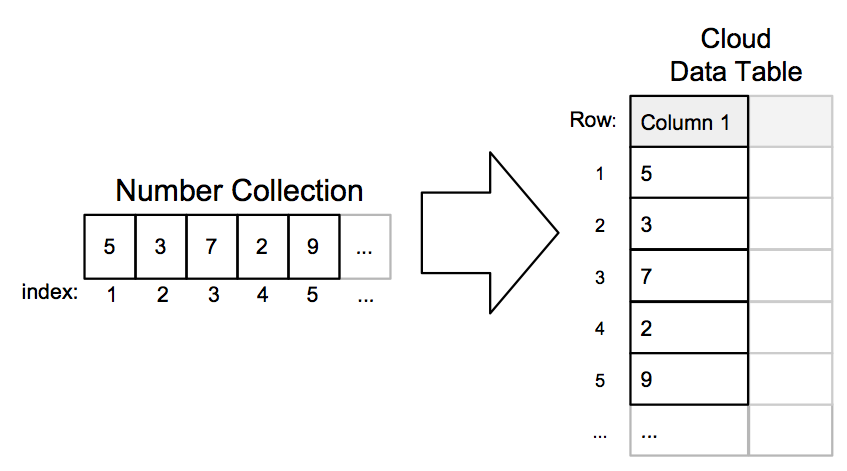
\includegraphics[width=250pt]{images/convertCollectionToTable}
\nocaptionrule
\caption{Conversion from Number Collection to Cloud Data Table}
\label{fig:ncToCDT}
\end{center}
\end{figure}


For these reasons, we automated this refactoring. 

Table~\ref{tab:refactoringsFormative} lists the total number of refactorings that we applied as part of our formative study.

\begin{table}[htdp]

\begin{center}
\begin{tabular}{|c|c|c|c|}
\hline
App  & Primitive & Local Table to   & Collection\\
 Name &  to Cloud  &  Cloud Table  & to Cloud \\
\hline
MileageTracker & 2 & 0 & 1\\
\hline
Buisness Manager+ & 0 & 0 & 5\\
\hline
CliffHangers & 8 & 0 & 2\\
\hline
My Assignments & 0 & 1 & 0\\
\hline
\hline
\textbf{Total} & 10 & 1  & 8 \\
\hline
\end{tabular}
\end{center}
\nocaptionrule
\caption{ Refactorings used in the formative study}
\label{tab:refactoringsFormative}
\end{table}%


\begin{table*}[htb!]
\centering
\begin{center}
\begin{tabular}{|c|c|c|}
 \hline
Number Collection Operations & Cloud Table Operations & Transformation Type\\
 \hline
 \hline
\code{clear} & \code{clear} & Direct \\
  \hline
  \code{count} & \code{count} & Direct \\
  \hline
\code{post to wall} & \code{post to wall} & Direct \\
\hline
\code{add} & \code{add row} & Indirect \\ 
\hline
\code{at} & \code{row at} & Indirect \\
\hline
\code{set at} & \code{row at$\rightarrow$valueName} & Indirect \\
\hline
\code{remove at} & \code{row at$\rightarrow$deleteRow} & Indirect \\
\hline
\code{insert at} & \code{row at$\rightarrow$value} & Indirect \\
\hline
\code{add many} & NONE & Injected Function \\
\hline
\code{avg} & NONE & Injected Function \\

\hline
\code{contains} & NONE & Injected Function \\
\hline

\code{index of} &NONE  & Injected Function \\

\hline
\code{max} &NONE  & Injected Function \\
\hline
\code{min} & NONE & Injected Function \\

\hline
\code{random} &NONE  & Injected Function \\
\hline
\code{remove}  & NONE & Injected Function \\

\hline
\code{reverse} &NONE  & Injected Function \\

\hline
\code{sort} & NONE &  Injected Function \\
\hline
\code{sum} & NONE &  Injected Function \\
\hline

\end{tabular}
\nocaptionrule
\caption{\texttt{Number Collection} API's and corresponding \texttt{Cloud Data Table} Operations. }
\label{tab:mappingTable}
\end{center}
\end{table*}%



\section{Automated Refactoring}
\label{sec:Refactoring}
This section presents our automated refactoring which converts from a local \NC{} to a \code{Cloud Data Table}. 
\FB{This refactoring is composed of several transformations.  The transformations are the individual changes that \tool must apply to the program in order to accomplish this refactoring. }
We implemented the refactoring in a tool, \tool, which itself is a \TD app.

Section~\ref{sec:workflow} presents the workflow of using the tool. Section~\ref{sec:preconditions} presents the preconditions that must be true
before applying the refactoring. Section~\ref{sec:transformations} presents the three kinds of transformations needed to perform the refactoring.


\subsection{Workflow}
\label{sec:workflow}
\tool is implemented as a \TD app.  It can be run using the \TD platform like any other \TD app.  Once it is run, the app first prompts the user to select a script on which to perform the refactoring.  Once the user has selected a script, \tool will display all the possible refactoring targets for the chosen script, and allow the user to choose which \NC they wish to convert to a \CDT. \tool will then perform all the needed transformations on the selected \NC in an automated fashion.  

\subsection{Preconditions}
\label{sec:preconditions}
In the current implementation of \TD, there are some differences in how \NC{}s and \CDT{}s are treated.
For example, an instance of a \NC{} can be passed as an argument or returned from a \TD function.  However, \CDT{}s cannot be passed as function arguments, or returned from functions.  Also, \NC{}s can be assigned to a variable, where as \CDT{}s cannot.  Based on these differences, we developed two preconditions that must be met before \tool can perform a refactoring.  These preconditions are inherent to how the \TD language works, not limitations of our tool.   

\POne  A \NC{} instance must not be passed as an argument or returned from a function. 

\PTwo A \NC{} instance must not be assigned to a variable.

\subsection{Transformations}
\label{sec:transformations}

There are four categories of transformations to refactor \NC{} to \code{Cloud Data Tables}: 
(i) creating \CDT{} data structure, (ii) direct mapping of APIs, (iii) indirect mapping of APIs, and (iv) injected function to augment missing APIs. Table~\ref{tab:mappingTable} displays the mapping between the APIs of the two data types.

We will illustrate the transformations using simplified code snippets from the MileageTracker app that we introduced in the Formative Study (see Section~\ref{sec:Formative}), an app that enables users to track their fuel usage. Figure~\ref{fig:codeTransformations} shows the code before and after the refactoring. The left column shows the original code. 
Line 1 shows the declaration of the \code{MileageRecord} \NC{}, which is the target of the refactoring. We show four functions to display all mileage record, clear existing mileage record, add a new entry to the mileage collection, and compute and display the average mileage. \\

\begin{figure*}
   \centering
    \mbox{
      \lstset{
	  language=Java, numbers=left, keywordstyle=\color{blue}, commentstyle=\color{red}, stringstyle=\color{black}, basicstyle=\scriptsize, tabsize = 2, moredelim=[is][\underbar]{_}{_}
      }
      \subfigure[before]{
      \lstinputlisting[]{src/in/TouchDevelopBefore.txt}
      \label{fig:aicOverload}
      }
      \hspace{0.2in}
      \subfigure[after]{
      \lstinputlisting[]{src/out/TouchDevelopAfter.txt}
      \label{fig:lambdaOverload}
      }
    }
    \caption{Relevant code from Mileage Tracker app. The left-hand side shows the original app, whereas the right-hand side shows the refactored code. The modified code is underlined, and the \texttt{avg} is a newly injected function.}
    \label{fig:codeTransformations}
\end{figure*}


\myParagraph{Create \texttt{Cloud Data Table} data structure: }
Lines 1-3 of the right-hand side of Figure~\ref{fig:codeTransformations} show the newly created data structure, \code{MileageRecordTable}. We append the \code{Table} to the end of the name for clarity. This \code{Table} contains one column, \code{MileageRecordColumn}. We will use this column to store the values that were originally stored in the \code{MileageRecord} collection.
\\


\myParagraph{Direct Transformations: } The simplest transformations are those when the mapping from the \NC{} to \CDT APIs is one-to-one and both data types use the same name (e.g., \code{post to wall}). In this case, the transformation consists of simply replacing the receiver object. 
Figure~\ref{fig:codeTransformations}~(a) line 8 shows the API call before the transformation, while Fig.~\ref{fig:codeTransformations}~(b) line 
8 shows the code after the transformation.\\

\myParagraph{Indirect Transformations: }
Indirect Transformations are more complex than Direct Transformations, and cannot be performed with a simple find-and-replace technique. We use Indirect Transformations when the same functionality can be accomplished in both data types, but the APIs are different: the cardinality and/or the name is different. Sometimes, the transformation maps one API call from the \NC{} into a sequence of API calls from the \CDT{}. In addition, sometimes it turns a function call into an assignment, further increasing complexity.

One example of an Indirect Transformation is shown in Figure~\ref{fig:codeTransformations}. 
The function \code{AddMileageToRecord} adds a number to the \code{MileageRecord} \NC{}. Line 26 in column (a) shows \code{Mileage} being added via the API call \code{add}.
In order to correctly perform the transformation, \code{Mileage} now needs to be added to the \code{Cloud Data Table} \code{MileageRecordTable}.
This becomes a two step process. Step 1 is to add a new row to the \CDT, and step two is to assign the value of \code{Mileage} to that row. This is shown in column (b) lines 26-27. \\


\MyParagraph{Injected Function Transformations: } 
We used Injected Function Transformations when some API functionality in \NC{} cannot be replicated using APIs from \CDT{}.
In order to transform such missing APIs, \tool inserts Injected Functions that provide the same functionality.  
Since \TD does not allow \CDT{}s to be passed to functions, but instead must be used as a global variable, \tool cannot create generic functions to replicate the API functionality.  
Instead, it must inject a function for each \CDT that has been created as a result of a refactoring. \FB{We developed a template for each Injected Function Transformation. These templates have ``holes'' and \tool then fills up these ``holes'' with the relevant table name and column name.  Thus \tool generates these Injected Functions fully automatically.}

One example of an Injected Function Transformation is shown in Fig~\ref{fig:codeTransformations}~(a) on lines 32-33.
The function \code{DisplayAvgMileage} calculates the average value of all contents of \code{MileageRecord}, and then displays it. 
Once \tool refactors the program to use a \CDT to store the data, there is no longer an API call that will calculate the average value 
of all contents of a \CDT. Instead, \tool must introduce the injected function \code{MileageRecordTable avg} (see Fig.~\ref{fig:codeTransformations}~(b) lines 36-45) that will compute the average of all the values in the \code{MileageRecordTable}.  
Now the API call in \code{DisplayAvgMileage} is transformed to call this \code{avg} injected function instead, as seen in Fig.~\ref{fig:codeTransformations}~(b), line 32.

\FB{Another example of an Injected Function Transformation is shown in Fig~\ref{fig:MaxCustomTransformationTransformations}.  Column (a) shows the template for the function that calculates the maximum value of a \CDT.  Column (b) shows the same function once it has been injected in the Mileage Tracker app. } \\
\MyParagraph{Concurrency: } 
\FB{Since multiple users can access the cloud data at the same time and perform updates concurrently, one needs to worry about the atomicity of compound operations in our Injected Functions.  However, \TD guarantees atomicity at the function level, thus our Injected Functions will execute atomically.}


\begin{figure*}
   \centering
    \mbox{
      \lstset{
	  language=Java, numbers=left, keywordstyle=\color{blue}, commentstyle=\color{red}, stringstyle=\color{black}, basicstyle=\scriptsize, tabsize = 2, moredelim=[is][\underbar]{_}{_}
      }
      \subfigure[Template Function]{
      \lstinputlisting[]{src/in/MaxBeforeRefactoring.txt}
      }
      \hspace{0.2in}
      \subfigure[Injected Function]{
      \lstinputlisting[]{src/out/MaxAfterRefactoring.txt}
      }
    }
    \caption{Template showing the injected function \texttt{max}. The left hand-side shows the template with ``holes'', whereas the right-hand side shows the function instantiated to use the \texttt{MileageRecordTable}.}
    \label{fig:MaxCustomTransformationTransformations}
\end{figure*}


\subsubsection{Tool Limitations}
The current version of \tool does not support the injected function transformation needed to transform the API call \code{add many}.  We believe that this function could be implemented but it remains as future work. 

\subsubsection{Implementation}
\FB{\tool refactors \TD scripts \emph{in place}.  First, \tool retrieves the source of the target app as an  Abstract Syntax Tree (AST) stored in JSON format from the \TD script bazaar.  It then transforms the AST as needed.  Once all the transformations are performed, \tool completes the refactoring by saving the new AST for the target app.}


\section{Evaluation}
\label{sec:evaluation}
To determine if \tool is useful we ask the following research questions.\\
Q1:  \textbf{APPLICABILITY}:  How applicable is the refactoring?\\
Q2:  \textbf{EFFORT}: How much effort is saved by \tool when refactoring?\\
Q3:  \textbf{ACCURACY}: How accurate is \tool when performing a refactoring?\\
 
\subsection{Methodology}

To create a corpus, we wrote queries against a database of all publicly available scripts in the \TD script bazaar. We wanted to collect popular and mature scripts. 
Thus, our query returned top scripts (based on the number of times that each script was executed) 
that contained a \NC{}. We retained the top \numScripts scripts.

Table~\ref{table:CorpusData} provides details about our corpus.  We report the size in non-blank source lines of code (SLOC) and complexity in number of functions.  We also report the number of times the apps were run by the \TD community, as well as the number of installations. Notice that a user can run an app without installing it in the user profile; this feature allows a \TD user to try out an app before installing it.

\begin{table}[htdp]
\begin{center}
\begin{tabular}{lclclc|c|c|}
\\
\hline
 & Average & Max & Std Dev & Total\\
\hline
SLOC & 403 & 2,526 & 483 & 47,185 \\
Functions & 21 & 121 & 26 & 2,502 \\
App Runs & 46 & 750 & 127 & 5,350 \\
App Installations & 5 & 125 & 18 & 635 \\

\end{tabular}
\nocaptionrule
\caption{Corpus Characteristics}
\label{table:CorpusData}
\end{center}
\end{table}%
 

Table~\ref{table:UsageOfAPIS} shows the total usage of the \NC APIs in our corpus.  For each API we report the total number of call sites in our corpus, as well as the percentage of call sites for the total API calls for \NC.


\begin{table}[htdp]
\begin{center}
\begin{tabular}{lclclc|}
\\
\hline
API Name & \# Call Sites & \% of total API Call Sites \\
\hline
At & 1010 & 39.25 \\
Set At & 632 & 24.56 \\
Add & 532 & 20.68 \\
Count & 109 & 4.24 \\
Contains & 107 & 4.16 \\
Clear & 84 & 3.26 \\
Remove At & 53 & 2.06 \\
Sum & 12 & 0.47 \\
Avg & 10 & 0.39 \\
Sort & 8 & 0.31 \\
Min & 4 & 0.16 \\
Post To Wall & 4 & 0.16 \\
Reverse & 4 & 0.16 \\
Max & 3 & 0.12 \\
Random & 1 & 0.04 \\


\end{tabular}
\nocaptionrule
\caption{Usage of Number Collection API reported in number of call sites}
\label{table:UsageOfAPIS}
\end{center}
\end{table}%

We ran the refactoring in batch mode. From each script in our corpus, our tool randomly selects one \NC{} as the target for refactoring. 

In order to determine the applicability of \tool, we report the number of scripts that our tool was able to refactor successfully, as well as the number of each kind of transformations performed inside a refactoring.

In order to determine the effort saved by using this refactoring tool we record the number of seconds each refactoring took. 

In order to validate the accuracy of \tool, we randomly chose \numManual scripts from the corpus of \numScripts refactored scripts. We ran the scripts and exercised the features for three minutes before and after each refactoring to ensure that the refactorings did not change the scripts' runtime behavior. Indeed, we did not observe any runtime differences before and after the refactoring. 

In addition to running these \numManual scripts we also carefully inspected the refactored code. We counted transformations that \tool
(i) applied correctly, (ii) applied incorrectly, and (iii) missed. 
\FB{The first two authors manually refactored \numManual scripts, and created a set of transformations for these refactorings.  We define this set of transformations that an expert would apply as our \emph{golden standard}.  For each transformation that \tool applied, we manually compared the result of the automated transformation with the golden standard to determine if that transformation had been applied correctly. 
We define a {\it TruePositive} as a transformation that \tool identified and applied correctly.   
We define {\it FalsePositive} as a transformation that \tool applies to the code, but it is not part of the golden standard. In other words, \tool transformed code that should not have been transformed.
We define a {\it FalseNegative} as a transformation that \tool did not apply, but it is in the golden standard. In other words, \tool missed applying a needed transformation.
}
 
 Using these metrics we calculate precision and recall for \tool, using the standard definitions:
\[precision = \frac{|True Positive|}{|True Positive|+|False Positive|}\]

\[recall = \frac{|True Positive|}{|True Positive|+|False Negative|}\]

\subsection{Results}

Next we present the results for each of the three research questions.


\textbf{Applicability: } 
Table~\ref{table:totalScripts} shows the results for running \tool on \numScripts scripts. 
Out of the \numScripts scripts that \tool attempted to refactor, 116 (94\%) met the preconditions for the refactoring.

Only 7 scripts were unable to be refactored. Out of these, 4 scripts did not meet precondition \POne (the \NC{} was passed as an argument to a function), and 1 did not meet precondition \PTwo (\NC{} was assigned to a local variable). The remaining 2 scripts exposed a limitation of the current implementation of \tool (they were using a currently unsupported function, \code{add many}). 
Thus, we think that our refactoring is widely applicable to \TD scripts that contain the \NC{} data type.  
\begin{table}[htdp]
\begin{center}
\begin{tabular}{ll} \\
\hline
Total Scripts & \numScripts \\
Number Successfully Refactored & 116 \\
Failed Precondition \POne & 4 \\
Failed Precondition \PTwo & 1\\
Tool Limitations & 2\\
\end{tabular}
\nocaptionrule
\caption{Total Scripts Refactored}
\label{table:totalScripts}
\end{center}
\end{table}%

\textbf{Effort:}  
Table~\ref{table:avgTrans} shows the number of transformations performed per each refactoring. 
 The first three rows show the type of these transformations (i.e., direct, indirect, and injected function). 
 The fourth row shows the total for all types of transformations, while the last row shows the running time for each refactoring.

The first column shows the average per script, while the last column shows the total for all the scripts.  Each script had, on average, 24 transformations applied in 3 seconds. Given that the \TD editing experience is optimized for small screens on touch devices, our refactoring tool saves significant effort.

Moreover, most of these transformations are non-trivial. Figure~\ref{fig:transformations_pieChart} shows the percentage of each kind of transformation applied. By far the most common transformation kind is Indirect Transformation, which involve mapping one API method call to a sequence of one or more API method calls that do not share a common name with the original method. Thus, we believe that automation saves significant effort.

\begin{table}[htdp]
\begin{center}
\begin{tabular}{lclclclclc||c|}

 & Avg & Max & Std Dev & Total\\
\hline
Refactorings & 1.84 & 8 & 1.38 & 211 \\
\hline
Direct Trans & 2.22 & 30 & 4.45 & 249\\

Indirect Trans & 19.88  & 466 & 56.62 & 2227\\

Injected Function & 2.20 & 30 & 5.01 & 246 \\
\hline
Total Trans & 24.30 & 466 & 56.56 & 2722 \\
\hline
Time [sec] & 2.64 & 27 & 5.18 & 296\\


\end{tabular}
\nocaptionrule
\caption{Refactorings Applied Per Script}
\label{table:avgTrans}
\end{center}
\end{table}%

\begin{figure}[htbp!]
\begin{center}
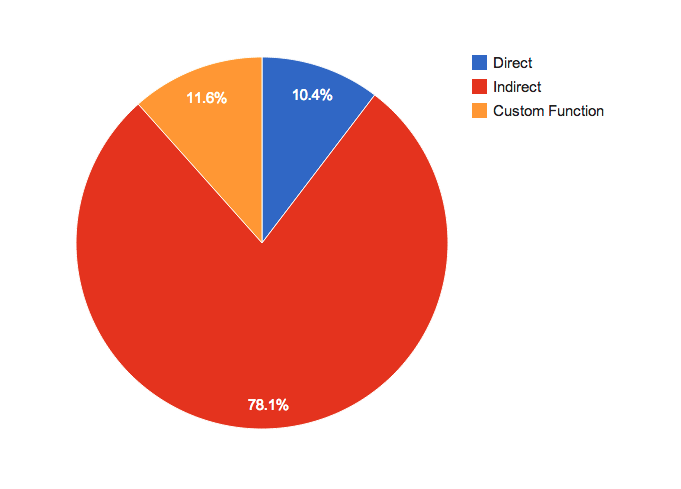
\includegraphics[width=250pt]{images/TransformationsChart}
\nocaptionrule
\caption{Transformations by Percentage}
\label{fig:transformations_pieChart}
\end{center}
\end{figure}

\textbf{Accuracy:}

By manually checking refactorings applied in \numManual scripts, we found \tool's \emph{precision} to be 100\% and its \emph{recall} 94\%. This means that all the transformations that \tool applied are correct. However, \tool missed 8 potential transformations out 145 transformations that it should have applied. We identified the root cause in our current implementation, and we expect a future version will fix this. 

\subsection{Threats to validity}
\textbf{Construct Validity:}  Do our metrics indeed measure the advantages of using \tool? Can we measure development effort by simply counting the time and number of transformations per refactoring? Ideally, we would have performed an experiment with real \TD developers and observe them while refactoring. However, given the cutting edge nature of the Cloud Data Types, we could not find such developers. Thus, we chose to use indirect metrics, as it is commonly done in the literature~\cite{Gyori:Lambdaficator,Wloka:Reentrancer}. 
Second, are we sure that the performed refactorings are accurate? Ideally, we should have run tests before and after each refactoring. However, very few scripts in \TD have any tests at all. In order to mitigate this we manually inspected a random set of \numManual apps and exercised their functionality to determine that the runtime behavior did not change.

\textbf{Internal Validity:}  How did we mitigate bias during manual inspection? We randomly sampled from the set of our corpus, until we had sampled from a variety of app domains. Also, we carefully constructed the set of transformations in the golden standard \emph{before} we applied \tool. The authors are all experts on the \TD platform.

Also, the corpus that we used in the evaluation predates the introduction of Cloud Data Types, and thus the developers were unaware of our later study and could not bias their code to help \tool. 

\textbf{External Validity:}  Do our results generalize? For our corpus, we used \numScripts of the most commonly run scripts, but we put no restrictions on the type of the scripts.  Our corpus includes scripts from various domains: entertainment, sports, games, education, productivity, etc. Moreover, the apps in our corpus are developed by 83 authors from a diverse end-user community. We do not foresee any reasons why our results would not generalize to other \TD apps.  
\FB{Currently there is no widely accepted standard for cloud data types.  In order for our results to generalize, cloud storage providers will first need to agree on Cloud Data Storage standards.}

\textbf{Reliability:} Is our evaluation reliable? The apps that we used to evaluate our tool are all available on the \TD bazaar, and \tool is published on the \TD website. All these URLs are available on our webpage: \\
\url{http://web.engr.oregonstate.edu/~hiltonm/Cloudifier}




\section{Related Work}
\label{sec:relatedWork}

We group the related work in the following categories: (i) cloud-related refactorings, (ii) multi-user apps, and (iii) tools for the end-user development community. \\

\MyParagraph{Cloud-related refactoring:}
There is a lot of research on generic topic of refactoring. While the original research was using refactoring to improve the design of existing programs, the more recent work used refactoring techniques to retrofit 
concurrency~\cite{wloka2009refactoring,dig2009refactoring}, functional features~\cite{Gyori:Lambdaficator}, etc.
As far as we know, we present the first automated tool to introduce mobile cloud computing via an automated refactoring tool.

The closest research to our current work is by Kwon and Tilevich~\cite{kwon2013cloud} who proposed \emph{Cloud Refactoring}, a tool to refactor methods of an enterprise application system into services that can be  ported to the cloud. Their tool also determines if a method is a good candidate for refactoring using static and dynamic analysis. However, even though their tool automatically refactors methods into services, the programmer must still move them to the cloud manually.  
Our tool, \tool, performs the refactoring fully automatically, including moving data to the cloud.  

Strauch et al.~\cite{strauchmigrating} describe a methodology for refactoring applications to move local data to cloud data. They propose several cloud data patterns, and describe migration scenarios for these patterns. Although this work provides a methodology at a high level, the application of the refactoring is completely manual and left up to the programmer. 
Ling et al.~\cite{ling2010refactoring} describe a systematic refactoring approach 
using category theory to formally define an approach to convert Object Oriented systems 
into Service-Oriented Architecture systems. 
Our work is different from these in that we provide a tool to perform the refactoring in an automated manner.

Researchers have used many approaches to harness the power of the cloud.
One of the more common uses of the mobile cloud is to offload computing in order to make apps more energy efficient and thereby preserve battery life, such as Spectra~\cite{flinn2002balancing}, Slingshot~\cite{su2005slingshot}, and MAUI~\cite{cuervo2010maui}.  
Kwon and Tilevich~\cite{kwon2012energy} proposed an approach to offload computation to the cloud to save battery life that is tolerant to network outages or unavailability.

CloudCone~\cite{chun2011clonecloud} also attempts to harness the power of mobile cloud computing, but their approach is significantly different then ours in that they create clones on the cloud, and then move the execution of the application as well as it's state between the cloud and the device.  \\

\MyParagraph{Multi-user apps:}
Many have studied multi-user apps in the following domains: collaboration~\cite{Yuill:multiuserColab, Lopez-Gulliver:imageprocessing}, gaming~\cite{Leichtenstern:multiuserGames}, Geospatial Applications~\cite{Forlines:geospatial} (e.g., Google earth), information sharing~\cite{Nacenta:2012:LMM:2307798.2307816}, and music~\cite{Sorensen:2012:ISM:2399016.2399094}. This research focuses on how multi-user technologies impact human interactions. In contrast, we are focused on the technical challenges of refactoring from single to multi-user apps. \\

\MyParagraph{End-user Development community:}
Lewis et al.~\cite{lewis2009report} describe the need of End User Programming tools to make End User Programming more acceptable.  

\TD is a programming platform developed by Microsoft Research that allows hobbyist, novice programmers and end users  to program \emph{on} their phone for their phone.  There are other programming environments that are targeted to a similar audience, including:  App Inventor~\cite{Wolber}, Scratch~\cite{maloney2010scratch}, Alice~\cite{cooper2010design}, and Greenfoot~\cite{kolling2010greenfoot}. 
Our recent work~\cite{badame2012refactoring} provides refactoring tools for users of Excel. 
However, our current paper is the first paper to engage the mobile end-user in a refactoring workflow.

\TODO{DANNY: ADD RELATED WORK ABOUT REFACTOR TO TABLE }

\section{Conclusion}
\label{sec:conclusions}
Mobile cloud computing can be harnessed to enable rich access to data. 
In this paper we presented a formative study to convert \numFormative apps to use the \TD cloud data types. 
Based on these lessons, we designed, implemented, and evaluated a tool,  \tool,  to refactor local data types into cloud data types.  
Our empirical evaluation on \numScripts real apps, shows that the tool is applicable, relevant, and saves human effort.
Using our refactoring tool in combination with a well designed, powerful end-user programming platform (\TD) can enable even novice programmers to take advantage of the power of the cloud.


%suprising. 

% We recommend abbrvnat bibliography style.

\bibliographystyle{abbrvnat}

% The bibliography should be embedded for final submission.

\bibliography{refs}


\end{document}

%                       Revision History
%                       -------- -------
%  Date         Person  Ver.    Change
%  ----         ------  ----    ------

%  2013.06.29   TU      0.1--4  comments on permission/copyright notices

